\section{Ingestion module for the MPL\_ORBPRE file}

This sections describes the ingestion module for inserting the orbit prediction of the satellites generated by \acrshort{fos}.

The associated ingestion processor is:

\begin{itemize} 

\item \textbf{s2boa.ingestions.ingestion\_orbpre.ingestion\_orbpre}
  
\end{itemize}

This module uses the following \acrshort{dim} signatures:

\begin{itemize} 

\item \textbf{ORBPRE}: data corresponding to the orbit prediction of the satellites generated by \acrshort{fos} used for adjusting the timing of the planning events which are using the operations angle.

\item \textbf{CORRECTED\_NPPF\_XXX}: data corresponding to the planning of operations commanding the satellite corrected by the available orbit prediction data.

\item \textbf{COMPLETENESS\_NPPF\_XXX}: data corresponding to the definition of planning completeness used for analysis.
  
\end{itemize}

Where XXX is the corresponding satellite id.

The figure \ref{fg:structure_ingestion_orbpre} shows a simplified diagram of the structure of events inserted (associated structure of values not included for simplicity).

\begin{figure}[H]
  \begin{center}
	\centering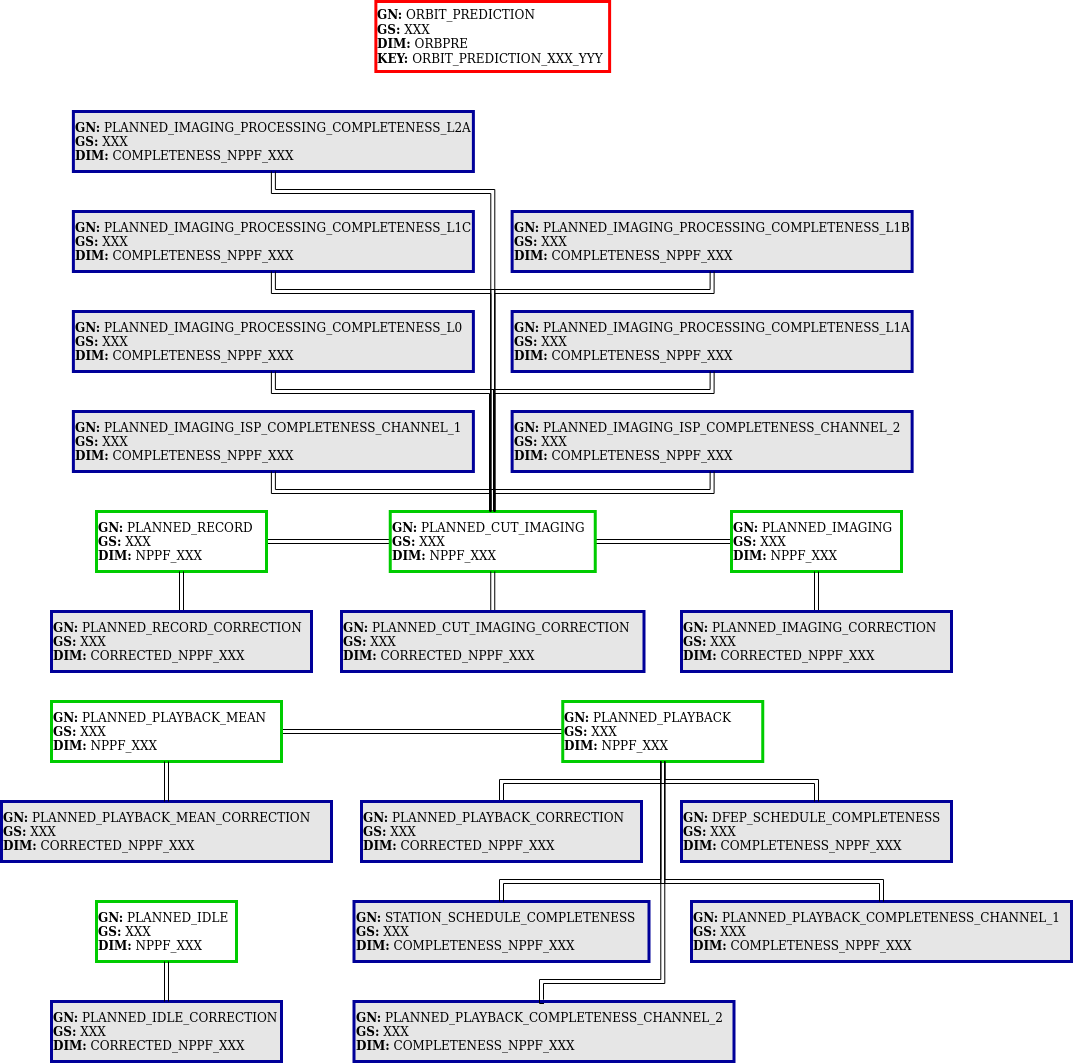
\includegraphics[width=150mm]{../fig/structure_ingestion_orbpre.png}
	\caption{Structure of events inserted by the ingestion module for the MPL\_ORBPRE file}
	\label{fg:structure_ingestion_orbpre}
  \end{center}
\end{figure}

Where YYY is the orbit number.

The table \ref{tb:description_events_ingestion_orbpre} shows the description of the events inserted by the ingestion.

\begin{landscape}
\begin{longtable}{|M{0.15\linewidth}|M{0.05\linewidth}|M{0.10\linewidth}|M{0.10\linewidth}|M{0.15\linewidth}|M{0.15\linewidth}|M{0.15\linewidth}|}
\hline \textbf{Gauge name} & \textbf{Gauge system} & \textbf{DIM signature} & \textbf{Insertion mode} & \textbf{Description} & \textbf{Start} & \textbf{Stop} \\ \hline
\textbf{ORBIT\_PREDICTION} & XXX & ORBIT\_PREDICTION\_XXX\_YYY & EVENT\_KEYS (insert) [KEY: ORBIT\_PREDICTION\_XXX\_YYY] & Event for representing the \textbf{orbit predition information of a specific orbit} & UTC time related to the ANX of orbit N & UTC time related to the ANX of orbit N + 1 \\ \hline
\textbf{***\_CORRECTION} & XXX & \- CORRECTED\_NPPF\_XXX & ERASE\_and\_REPLACE (insert\_and\_erase) & Event for representing the \textbf{planning events corrected using the orbit prediction events} & Start of the planned event corrected using the ORBPRE & Stop of the planned event corrected using the ORBPRE \\ \hline
\textbf{DFEP\_SCHEDULE\_COMPLETENESS} & XXX & \- COMPLETENESS\_NPPF\_XXX & ERASE\_and\_REPLACE (insert\_and\_erase) & Event for representing the \textbf{expectation of the DFEP schedule} & Corrected start of the planned playback + 2s (SAD/HKTM) or + 9s (MSI); (if start \textgreater  stop) Corrected stop of the planned playback - 4s & Start (SAD/HKTM) or Corrected stop of the planned playback - 9s (MSI); (if start \textgreater  stop) Corrected stop of the planned playback - 3s \\ \hline
\textbf{STATION\_SCHEDULE\_COMPLETENESS} & XXX & \- COMPLETENESS\_NPPF\_XXX & ERASE\_and\_REPLACE (insert\_and\_erase) & Event for representing the \textbf{expectation of the Station schedule} & Corrected start of the planned playback + 2s (SAD/HKTM) or + 9s (MSI); (if start \textgreater  stop) Corrected stop of the planned playback - 4s & Start (SAD/HKTM) or Corrected stop of the planned playback - 9s (MSI); (if start \textgreater  stop) Corrected stop of the planned playback - 3s \\ \hline
\textbf{PLANNED\_PLAYBACK\_COMPLETENESS\_CHANNEL\_1} & XXX & \- COMPLETENESS\_NPPF\_XXX & ERASE\_and\_REPLACE (insert\_and\_erase) & Event for representing the \textbf{expectation of the planned playbacks using the channel 1} & Corrected start of the planned playback + 2s (SAD/HKTM) or + 9s (MSI); (if start \textgreater  stop) Corrected stop of the planned playback - 4s & Start (SAD/HKTM) or Corrected stop of the planned playback - 9s (MSI); (if start \textgreater  stop) Corrected stop of the planned playback - 3s \\ \hline
\textbf{PLANNED\_PLAYBACK\_COMPLETENESS\_CHANNEL\_2} & XXX & \- COMPLETENESS\_NPPF\_XXX & ERASE\_and\_REPLACE (insert\_and\_erase) & Event for representing the \textbf{expectation of the planned playbacks using the channel 2} & Corrected start of the planned playback + 2s (SAD/HKTM) or + 9s (MSI); (if start \textgreater  stop) Corrected stop of the planned playback - 4s & Start (SAD/HKTM) or Corrected stop of the planned playback - 9s (MSI); (if start \textgreater  stop) Corrected stop of the planned playback - 3s \\ \hline
\textbf{PLANNED\_IMAGING\_ISP\_COMPLETENESS\_CHANNEL\_1} & XXX & \- COMPLETENESS\_NPPF\_XXX & ERASE\_and\_REPLACE (insert\_and\_erase) & Event for representing the \textbf{expectation of the planned imaging using the channel 1} & Corrected start of the planned imaging + 10s; (if start \textgreater  stop) Corrected stop of the planned imaging - 12s & Corrected stop of the planned imaging - 10s; (if start \textgreater  stop) Corrected stop of the planned imaging - 6s \\ \hline
\textbf{PLANNED\_IMAGING\_ISP\_COMPLETENESS\_CHANNEL\_2} & XXX & \- COMPLETENESS\_NPPF\_XXX & ERASE\_and\_REPLACE (insert\_and\_erase) & Event for representing the \textbf{expectation of the planned imaging using the channel 2} & Corrected start of the planned imaging + 10s; (if start \textgreater  stop) Corrected stop of the planned imaging - 12s & Corrected stop of the planned imaging - 10s; (if start \textgreater  stop) Corrected stop of the planned imaging - 6s \\ \hline
\textbf{PLANNED\_IMAGING\_PROCESSING\_COMPLETENESS\_L0} & XXX & \- COMPLETENESS\_NPPF\_XXX & ERASE\_and\_REPLACE (insert\_and\_erase) & Event for representing the \textbf{expectation of the processing of the planned imaging for the L0} & Corrected start of the planned imaging + 10s; (if start \textgreater  stop) Corrected stop of the planned imaging - 12s & Corrected stop of the planned imaging - 10s; (if start \textgreater  stop) Corrected stop of the planned imaging - 6s \\ \hline
\textbf{PLANNED\_IMAGING\_PROCESSING\_COMPLETENESS\_L1A} & XXX & \- COMPLETENESS\_NPPF\_XXX & ERASE\_and\_REPLACE (insert\_and\_erase) & Event for representing the \textbf{expectation of the processing of the planned imaging for the L1A} & Corrected start of the planned imaging + 10s; (if start \textgreater  stop) Corrected stop of the planned imaging - 12s & Corrected stop of the planned imaging - 10s; (if start \textgreater  stop) Corrected stop of the planned imaging - 6s \\ \hline
\textbf{PLANNED\_IMAGING\_PROCESSING\_COMPLETENESS\_L1B} & XXX & \- COMPLETENESS\_NPPF\_XXX & ERASE\_and\_REPLACE (insert\_and\_erase) & Event for representing the \textbf{expectation of the processing of the planned imaging for the L1B} & Corrected start of the planned imaging + 10s; (if start \textgreater  stop) Corrected stop of the planned imaging - 12s & Corrected stop of the planned imaging - 10s; (if start \textgreater  stop) Corrected stop of the planned imaging - 6s \\ \hline
\textbf{PLANNED\_IMAGING\_PROCESSING\_COMPLETENESS\_L1C} & XXX & \- COMPLETENESS\_NPPF\_XXX & ERASE\_and\_REPLACE (insert\_and\_erase) & Event for representing the \textbf{expectation of the processing of the planned imaging for the L1C} & Corrected start of the planned imaging + 10s; (if start \textgreater  stop) Corrected stop of the planned imaging - 12s & Corrected stop of the planned imaging - 10s; (if start \textgreater  stop) Corrected stop of the planned imaging - 6s \\ \hline
\textbf{PLANNED\_IMAGING\_PROCESSING\_COMPLETENESS\_L2A} & XXX & \- COMPLETENESS\_NPPF\_XXX & ERASE\_and\_REPLACE (insert\_and\_erase) & Event for representing the \textbf{expectation of the processing of the planned imaging for the L2A} & Corrected start of the planned imaging + 10s; (if start \textgreater  stop) Corrected stop of the planned imaging - 12s & Corrected stop of the planned imaging - 10s; (if start \textgreater  stop) Corrected stop of the planned imaging - 6s \\ \hline
\caption{Table describing the events associated to the ingestion}
\label{tb:description_events_ingestion_orbpre}
\end{longtable}
\end{landscape}

\section{Ingestion details}

This section describes some ingestion details for inserting the data. In particular:

\begin{itemize} 

\item The algorithm to correct the timing of the planning events
  
\end{itemize}

The algorithm to correct the timing of the planning events is as follows:

For every planning event:

\begin{itemize} 

\item Get satellite ID, start and stop orbits and start and stop angles.

\item Get the \acrshort{anx} time from the orbit prediction information covering the previous orbits and the following ones

\item Apply the following formula to the start and stop angles (\(\alpha\)) using the orbital period (p) and the corresponding \acrshort{anx} timing (t):

  \(sin_1 = sin(\alpha)\)

  \(sin_2 = sin(2*\alpha)\)

  \(cos_1 = cos(\alpha)\)

  \(cos_2 = cos(2*\alpha)\)

  \(cos_3 = cos(3*\alpha)\)

  Adjust angle to a circunference (perfect distribution in 360º):
  
  \(m = \alpha - 0.13175612 - 2*(-0.0001529)*sin_1 - 2*(-0.0660818)*cos_1 - 2*0.16855853*sin_2 - 2*(-0.0007759)*cos_2 - 2*0.0009872*cos_3 - 2*0.00687159*sin_2\)

  Transform angle to \(\delta\) time:
  
  \(s = (m * p)/360.0\)

  \(UTC time = t + s \)
  
\end{itemize}
